
\documentclass[17pt]{article}
\usepackage{enumitem}
\usepackage{amsmath}
\usepackage{mathtools}
\usepackage{amssymb}
\usepackage{tikz, ifthen}
\usepackage{algorithm}
\usepackage[noend]{algpseudocode}
\usepackage{ulem}
\usepackage{kbordermatrix}
\usetikzlibrary{matrix,calc}
\DeclarePairedDelimiter\norm{\lVert}{\rVert}%
\begin{document}

\title{ Mid Term Exam (Group MT-09)\\Machine Learning - 1 [CS/DS 864] }
\author{Darshan Bhat - MT2015038\\Keerthan Pai K - MT2015053}
\maketitle
Note: We have discussed with Group MT-03(Freeze Francis and Mohammed Haroon), but the representaions are different.
\\
\subsection*{Q.1}
The given description of $H_i's$ follows the structure of a feed-forward neural network with one hidden layer and one node in the output layer.\\\\
For given n input points, each $H_i$ hypothesis class can produce $G_{H_{i}}(n)$ labellings. In the extreme case, the labellings produced are all distinct at the output of hidden layer. Now if $H_1$ can produce $G_{H_{1}}(n)$ different labellings of n input points, and $H_2$ can produce $G_{H_{2}}(n)$ different labellings independent of $H_1$ class ,then together we have $G_{H_{1}}(n) \times G_{H_{2}}(n)$ different possible labellings of n points at maximum.\\\\
With k hypothesis classes at the hidden layer, total number of distinct labellings is upper bounded by $\prod_{i=1}^{k}G_{H_{i}}(n)$. Now these labellings are fed to the output layer with $H_0$ hypothesis class. Each input can now be labelled with one of the $G_{H_{0}}(n)$ labellings. This implies a total of 
$G_{H_{0}}(n) \times \prod_{i=0}^{k}G_{H_{i}}(n)$ labellings are possible at the output layer.\\\\
That is,
$$G_{H}(n) \leq \prod_{i=0}^{k}G_{H_{i}}(n)$$
We need to prove
$$d_{H} \leq 2D\log_{2}D$$
given that,
$$D > e\log_{2}D$$
Proof:
\begin{equation*}
\begin{aligned}
2^{d_{H}} & \leq \prod_{i=0}^{k} \left( \dfrac{e d_{H}}{d_{H_{i}}}\right)^{d_{H_{i}}}\\
&  \leq \prod_{i=0}^{k} \left( \dfrac{e d_{H}}{2}\right)^{d_{H_{i}}}\\
&  \leq  \left( \dfrac{e d_{H}}{2}\right)^{ \sum_{i=0}^{k} d_{H_{i}}}\\
\end{aligned}
\end{equation*}

$$2^{d_{H}} \leq \left( \dfrac{e d_{H}}{2}\right)^{D}$$
$$d_{H} \leq D \log_2\left( \dfrac{e d_{H}}{2} \right)$$
This holds for all valid $d_{H}$ values. We will prove our claim by contradiction.\\\\
Let $d_{H} > 2D \log_2 D$

i.e. $d_{H}=2D \log_2 D +1$, and we know that  $D > e \log_{2} D$\\
\begin{equation*}
\begin{aligned}
\therefore 2D \log_2 D + 1 
& \leq D \log_2 \left( \dfrac{e 2 D\log_2 D + e}{2} \right)\\
& \leq D \log_2 \left( \dfrac{2 e D \log_2 D + 2 e D \log_2 D}{2}\right) \\
& \leq D \log_2 \left( \frac{4 e D \log_2 D }{2}\right) \\
& \leq D \log_2 \left( 2 e D \log_2 D\right)\\
\implies 2 D \log_2 D &< D \log_2 \left( 2 e D \log_2 D\right)\\
2 \log_2 D &< \log_2 2 + \log_2 e + \log_2 D + \log_2 (\log_2 D)\\
log_2 D &< \log_2 2 + \log_2 e + \log_2 (\log_2 D)\\
\implies log_2 D &\leq \log_2(e \log_2 D)\\
\implies D &\leq e \log_2 D
\end{aligned}
\end{equation*}
This contradicts with the given $D > e\log_{2}D$.\\

Hence,
$$d_{H} \leq 2D\log_{2}D$$

%%%%%%%%%%%%%%%%%%%%%%%%%%%%%%%%%%%%%%%%%%%%%%%%%%%%%%%%%%%%%

\newpage

%%%%%%%%%%%%%%%%%%%%%%%%%%%%%%%%%%%%%%%%%%%%%%%%%%%%%%%%%%%%%
\subsection*{Q.2}

\textbf{2.a)}We can prove that H matrix is idempotent.
\\ $$H=X\left(X ^{T}X\right)^{-1}X ^{T}$$
$$H^{2}=X\left(X ^{T}X\right)^{-1}X ^{T}X\left(X ^{T}X\right)^{-1}X ^{T}$$
$$H^{2}=X\left(X ^{T}X\right)^{-1}(X ^{T}X)\left(X ^{T}X\right)^{-1}X ^{T}$$
$$H^{2}=X\left(X ^{T}X\right)^{-1}X ^{T}$$
$$H^{2}=H$$
Now consider,\\
$$Hx=\lambda x$$
$$H^{2}x=\lambda x$$
$$HHx=\lambda x$$
$$H\lambda x=\lambda x$$
$$\lambda Hx=\lambda x$$
$$\lambda^{2} x=\lambda x$$
$$(\lambda^{2}-\lambda) x=0$$
Solving for $\lambda$ gives $\lambda = 0$ and $\lambda = 1$.\\
\\
\\
\textbf{2.b)}\\
The proof is by induction on the size $n$ of the matrix $A$. The result is trivial for $n = 1$. Now let $n>1$ and assume the result is true for any matrix of size $n-1$.\\
\\
Let $\lambda$ be the eigenvalue of $A$, that is, $det(\lambda I - A) = 0$, then $\lambda I - A$ must be non-invertible. This means that there exist a non-zero real vector $u$ such that $A u = \lambda u$. We can always normalize $u$ so that $u^Tu = 1$. Thus, $\lambda = u^TAu$ is real. That is, the eigenvalues of a symmetric matrix are always real.\\
\\
Now consider the eigenvalue $\lambda_1$ and an associated eigenvector $u_1$. Using the Gram-Schmidt orthogonalization procedure, we can compute a $n\times(n-1)$ matrix $V_1$ such that $[u_1,V_1]$ is orthogonal. By induction, we can write the $(n-1)\times(n-1)$ symmetric matrix $V_1^TAV_1$ as $Q_1 \Lambda_1 Q_1^T$, where $Q_1$ is a $(n-1)\times(n-1)$ matrix of eigenvectors, and $\Lambda_1 = \mbox{\bf diag}(\lambda_2,\ldots,\lambda_n)$ are the $n-1$ eigenvalues of $V_1^TAV_1$. Finally, we define the $n\times (n-1)$ matrix $U_1 := V_1Q_1$. By construction the matrix $U := [u_1,U_1]$ is orthogonal.\\
\\
We have
\begin{equation*}
U^TAU = \left( \begin{array}{c} u_1^T\\ U_1^T \end{array}\right)A \left( \begin{array}{cc} u_1 & U_1 \end{array}\right) = \left( \begin{array}{cc} u_1^TAu_1 & u_1^TAU_1\\ U_1^TAu_1 & U_1^TAU_1 \end{array} \right) = \left( \begin{array}{cc} \lambda_1 & 0\\ 0 & \Lambda_1 \end{array}\right), 
\end{equation*}where we have exploited the fact that $U_1^TAu_1 = \lambda_1 U_1^Tu_1 = 0$, and $U_1^TAU_1 = \lambda_1$.\\
\\
We have exhibited an orthogonal $n\times n$ matrix $U$ such that $U^TAU$ is diagonal. This proves the theorem.\\
\\\\
\textbf{2.c)}\\
The trace of a matrix is the sum of its diagonal entries. This has the property that $\text{Tr}(AB)=\text{Tr}(BA)$ for any two matrices of same size. $X^TX$ is a $(p+1)\times(p+1)$ matrix.
\\\\
Now consider,
\begin{equation*}
\begin{aligned}
	\text{Tr}(H) &= \text{Tr}(X(X^TX)^{-1}X^T)\\
				 &= \text{Tr}((X^TX)^{-1}X^TX)\\
				 &= \text{Tr}(I_{p+1})\\
				 &= p+1\\
\end{aligned}
\end{equation*}
$$\text{Tr}(H) = \lambda_1 + \lambda_2 + ... + \lambda_{p+1}$$
Since $\lambda \in$ {0,1}, we can conclude that number of eigen values which are 1's is $p+1$. 

%%%%%%%%%%%%%%%%%%%%%%%%%%%%%%%%%%%%%%%%%%%%%%%%%%%%%%%%%%%%%

\newpage

%%%%%%%%%%%%%%%%%%%%%%%%%%%%%%%%%%%%%%%%%%%%%%%%%%%%%%%%%%%%%

\subsection*{Q.3}
To show that $X^tX$ is positive definite.\\
Consider,
$$v^{t}X^{t}Xv=(Xv)^{t}(Xv) \hspace{8cm}(1)$$
Let $Xv=z$ with the dimension $n \times 1$.\\
$$(1) \Rightarrow z^{t}z=||z||^{2}>0$$
So, $X^{t}X > 0$ and thus it is positive semi definite.\\
We can model linear regression as as a system of linear equations.
The vector equation is equivalent to a matrix equation of the form
 $$ X{\mathbf {w}}={ {y}}$$
where X is an $n \times p$ matrix, w is a column vector with p entries, and y is a column vector with n entries.
   $$X={\begin{bmatrix}x_{11}&x_{12}&\cdots &x_{1p}\\x_{21}&x_{22}&\cdots &x_{2p}\\\vdots &\vdots &\ddots &\vdots \\x_{n1}&x_{n2}&\cdots &x_{np}\end{bmatrix}},\quad {\mathbf {w}}={\begin{bmatrix}w_{1}\\w_{2}\\\vdots \\w_{p}\end{bmatrix}},\quad {\mathbf {y}}={\begin{bmatrix}y_{1}\\y_{2}\\\vdots \\y_{n}\end{bmatrix}}$$
Solution for such a system exist only if $\textbf{y}$ is in the column space of $\textbf{X}$. It may happend that there exist no solution. In such case we can find the best $\textbf{w}$ such that $\textbf{Xw}$  is closest to $\textbf{b}$ by using least squares approximation.\\
We know that $\textbf{Xw}$ is in the column space of $\textbf{X}$ and $\textbf{y}$ is not in the plane of $\textbf{Xw}$.This can be achieved only when $\textbf{Xw}$ is the projection of $\textbf{y}$  
\\
\begin{figure}[h!]
	\centering
	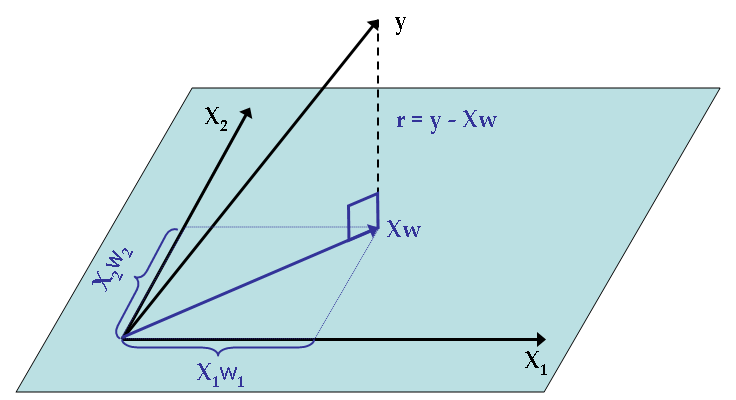
\includegraphics[width=90mm]{ols-regression-geometry.png}
	\caption{\label{convex}}
\end{figure}
$$\therefore \textbf{Xw} \perp (y-\textbf{Xw}) $$
$$\therefore (\textbf{Xw})^{t} \hspace{0.2cm}  (y-\textbf{Xw})=0$$
$$\textbf{w}^{t}\textbf{X}^{t} \hspace{0.2cm} (y-\textbf{Xw})=0 $$
$$\textbf{w}^{t}\textbf{X}^{t}y-\textbf{w}^{t}\textbf{X}^{t}\textbf{Xw}=0$$
$$\textbf{w}^{t}\textbf{X}^{t}y=\textbf{w}^{t}\textbf{X}^{t}\textbf{Xw}$$
$$\textbf{X}^{t}y=\textbf{X}^{t}\textbf{Xw}$$
$$\textbf{w}=(\textbf{X}^{t}\textbf{X})^{-1}\textbf{X}^{t}y$$
\\
\\
Alternatively, the closed form solution can be derived using the positive semidefinite property of the matrix $\boldsymbol X^TX$. Consider the loss function,
\begin{equation*}
\begin{aligned}
S({\boldsymbol {w }}) 
	&={\bigl \|}\mathbf {y} -\mathbf {X} {\boldsymbol {w }}{\bigr \|}^{2}\\
	&=(\mathbf {y} -\mathbf {X} {\boldsymbol {w }})^{\rm {T}}(\mathbf {y} -\mathbf {X} {\boldsymbol {w }})\\
	&=\mathbf {y} ^{\rm {T}}\mathbf {y} -{\boldsymbol {w }}^{\rm {T}}\mathbf {X} ^{\rm {T}}\mathbf {y} -\mathbf {y} ^{\rm {T}}\mathbf {X} {\boldsymbol {w }}+{\boldsymbol {w }}^{\rm {T}}\mathbf {X} ^{\rm {T}}\mathbf {X} {\boldsymbol {w }}
\end{aligned}
\end{equation*}\\
When $\mathbf X^{\rm T} \mathbf X$ is positive definite, the quantity
$$S(\boldsymbol{w}) = \mathbf y ^{\rm T} \mathbf y - 2\boldsymbol w ^{\rm T} \mathbf X ^{\rm T} \mathbf y + \boldsymbol w ^{\rm T} \mathbf X ^{\rm T} \mathbf X \boldsymbol w $$
can be written as
$$ \langle \boldsymbol w, \boldsymbol w \rangle - 2\langle \boldsymbol w, (\mathbf X^{\rm T} \mathbf X)^{-1}\mathbf X ^{\rm T} \mathbf y \rangle + \langle(\mathbf X^{\rm T} \mathbf X)^{-1}\mathbf X ^{\rm T} \mathbf y,(\mathbf X^{\rm T} \mathbf X)^{-1}\mathbf X ^{\rm T} \mathbf y \rangle+ C, $$
where  C  depends only on  $\mathbf y $ and  $\mathbf X $, and  $\langle \cdot, \cdot \rangle$  is the inner product defined by
 $$\langle x, y \rangle = x ^{\rm T} (\mathbf X^{\rm T} \mathbf X) y. $$
It follows that $ S(\boldsymbol{w})$  is equal to
$$\langle \boldsymbol w - (\mathbf X^{\rm T} \mathbf X)^{-1}\mathbf X ^{\rm T} \mathbf y,\boldsymbol w - (\mathbf X^{\rm T} \mathbf X)^{-1}\mathbf X ^{\rm T} \mathbf y \rangle+ C $$
and therefore minimized exactly when
$$\boldsymbol w - (\mathbf X^{\rm T} \mathbf X)^{-1}\mathbf X ^{\rm T} \mathbf y = 0.$$
Hence the the best value of w is,
$$\boldsymbol w = (\mathbf X^{\rm T} \mathbf X)^{-1}\mathbf X ^{\rm T} \mathbf y$$
%%%%%%%%%%%%%%%%%%%%%%%%%%%%%%%%%%%%%%%%%%%%%%%%%%%%%%%%%%%%%
\newpage
%%%%%%%%%%%%%%%%%%%%%%%%%%%%%%%%%%%%%%%%%%%%%%%%%%%%%%%%%%%%%
\subsection*{Q.4}
\textbf{4.a)} y is of the form $y = g(x) + \epsilon_x$.\\
Let $\mathbf{Y} = {\begin{bmatrix}y_{1}\\y_{2}\\\vdots \\y_{n}\end{bmatrix}}$\\\\
$$So,\: Y = g + \epsilon \hspace{9.5cm}(1)$$
where $\quad {\mathbf {g}}={\begin{bmatrix}g(x_1)\\g(x_2)\\\vdots \\g(x_n)\end{bmatrix}},\quad {\mathbf {\epsilon}}={\begin{bmatrix}\epsilon_{x_1}\\\epsilon_{x_2}\\\vdots \\\epsilon_{x_n}\end{bmatrix}}$\\\\
\begin{equation*}
\begin{split}
E &= (Y^T -w^TX^T)(Y - Xw)\\
    &= Y^TY - Y^TXw  - w^TX^TY + w^TX^TXw\\
\end{split}
\end{equation*}
To get optimal weights $\hat{w}$, $ \frac{\delta E}{\delta w} = 0$\\
$$i.e. -X^TY - X^TY + 2X^TX\hat{w} = 0$$
$$ X^TX\hat{w} = X^TY$$
$$ \therefore \hat{w} = (X^TX)^{-1}X^TY$$
From equation (1),
$$\hat{w} = (X^TX)^{-1}X^T(g+\epsilon)$$
Estimated output $\hat{y} = X\hat{w}$
$$\hat{y} = X(X^TX)^{-1}X^Tg+ X(X^TX)^{-1}X^T\epsilon$$
From the given data, $g = Xw^*$\\
So, 
$$\hat{Y} = X(X^TX)^{-1}X^T(Xw^*)+ X(X^TX)^{-1}X^T\epsilon$$
$\hspace{2.75cm}\hat{Y} = Xw* + \hat{H}\epsilon \hspace{6.5cm}$ (2)\\    
From the given data, $$ y = x^Tw^* + \epsilon$$
From (2) $\hat{y}$ at a given point $x$ will be
$$\hat{y} = x^Tw^* + x^T(X^TX)^{-1}X^T\epsilon$$
$$y - \hat{y} = \epsilon - x^T(X^TX)^{-1}X^T\epsilon$$\\
\textbf{4.b)}Let
   $${\mathbf {X}}={\begin{bmatrix}x_{1}\\x_{2}\\\vdots \\x_{n}\end{bmatrix}},
   \quad  \mathbf{A}= {\begin{bmatrix}
   		a_{11}&a_{12}&\cdots &a_{1n}\\
   		a_{21}&a_{22}&\cdots &a_{2n}\\
   		\vdots &\vdots &\ddots &\vdots\\
   		a_{n1}&a_{n2}&\cdots &a_{nn}					\end{bmatrix}}
	$$
We have,
\begin{equation*}
\begin{split}
x^TAx &= { {\begin{bmatrix}x_{1}&x_{2}&\cdots&x_{n}\end{bmatrix}}
	{\begin{bmatrix}
   		a_{11} &a_{12} &\cdots &a_{1n}\\
   		a_{21} &a_{22} &\cdots &a_{2n}\\
   		\vdots &\vdots &\ddots &\vdots\\
   		a_{n1} &a_{n2} &\cdots &a_{nn}
   	\end{bmatrix}}
	{\begin{bmatrix}x_{1}\\x_{2}\\\vdots\\x_{n}\end{bmatrix}}
}
  \\
	 &= { {\begin{bmatrix}x_{1}&x_{2}&\cdots&x_{n}\end{bmatrix}}
	{\begin{bmatrix}
   		a_{11}x_{1} + a_{12}x_{2} + \cdots + a_{1n}x_{n}\\
   		a_{21}x_{1} + a_{22}x_{2} + \cdots + a_{2n}x_{n}\\
   		\vdots\\
   		a_{n1}x_{1} + a_{n2}x_{2} + \cdots + a_{nn}x_{n}
   	\end{bmatrix}}
} \\
	 &= {\begin{split}	 
			& a_{11}x_{1}^2 + a_{12}x_{1}x_{2} +\cdots + a_{1n}x_{1}x_{n} +a_{21}x_{2}x_{1}+a_{22}x_{2}^2+\cdots + a_{2n}x_{2}x_{n}\\
			& +\cdots\cdots+a_{n1}x_{n	}x_{1}+\cdots+a_{nn}x_{n}^2 \hspace{7.25cm}(1)  
	 	\end{split}
}
   \\
\end{split}
\end{equation*}\\
Also,
$$xx^T = { 
	{\begin{bmatrix}x_{1}\\x_{2}\\\vdots\\x_{n}\end{bmatrix}}
	{\begin{bmatrix}x_{1}&x_{2}&\cdots&x_{n}\end{bmatrix}}	
} = \begin{bmatrix}
   		x_{1}^2 &x_{1}x_{2} &\cdots &x_{1}x_{n}\\
   		x_{2}x_{1} &x_{2}^2 &\cdots &x_{2}x_{n}\\
   		\vdots &\vdots &\ddots &\vdots\\
   		x_{n}x_{1} &x_{n}x_{2} &\cdots &x_{n}^2
   	\end{bmatrix}
$$
$$xx^TA = {
	{\begin{bmatrix}
   		x_{1}^2 &x_{1}x_{2} &\cdots &x_{1}x_{n}\\
   		x_{2}x_{1} &x_{2}^2 &\cdots &x_{2}x_{n}\\
   		\vdots &\vdots &\ddots &\vdots\\
   		x_{n}x_{1} &x_{n}x_{2} &\cdots &x_{n}^2
	   	\end{bmatrix}}
{\begin{bmatrix}
   		a_{11}&a_{12}&\cdots &a_{1n}\\
   		a_{21}&a_{22}&\cdots &a_{2n}\\
   		\vdots &\vdots &\ddots &\vdots\\
   		a_{n1}&a_{n2}&\cdots &a_{nn}					\end{bmatrix}}
}
$$
$$trace(xx^TA) = {\begin{split}	 
				& a_{11}x_{1}^2 + a_{21}x_{1}x_{2} +\cdots + a_{n1}x_{1}x_{n} +a_{12}x_{2}x_{1}+a_{22}x_{2}^2+\cdots + a_{n2}x_{2}x_{n}\\
				& +\cdots\cdots+a_{1n}x_{n	}x_{1}+\cdots+a_{nn}x_{n}^2 \hspace{6cm}(2)  
	 		\end{split}
	 	   }$$
Since A is symmetric, $a_{ij} = a_{ji}$\\
So, (1) = (2) that is,
$$x^TAx = tr(xx^TA)$$
Since Expectation E(.) and trace tr(.) both are linear operators,
\begin{equation*}
\begin{aligned}
tr[E[M]] &= \sum_{i} E[ M_{ii} ]\\
	     &=  E[ \sum_{i} M_{ii} ] \\
   	     &=  E[ tr [M] ] 
\end{aligned}
\end{equation*}
\textbf{4.c)} $x$ is a d-dimensional vector in $R^{d}$. We need to estimate the covariance matrix $E_{D}[xx^{T}]$ where expectation is over all possible datasets which is simply the expectattion of $xx^{T}$ in the domain of $x$. The matrix $xx^{T}$ will be of the order $d \times d$.

$$xx^T = {
      {	\begin{bmatrix}
          x_{1}^2 &x_{1}x_{2} &\cdots &x_{1}x_{d}\\
          x_{2}x_{1} &x_{2}^2 &\cdots &x_{2}x_{d}\\
          \vdots &\vdots &\ddots &\vdots\\
          x_{d}x_{1} &x_{p}x_{2} &\cdots &x_{d}^2
      	\end{bmatrix}
      }
	}
$$

$$E[xx^T] = {
      {  \begin{bmatrix}
           E[x_{1}^2] &E[x_{1}x_{2}] &\cdots &E[x_{1}x_{d}]\\
           E[x_{2}x_{1}] &E[x_{2}^2] &\cdots &E[x_{2}x_{d}]\\
           \vdots &\vdots &\ddots &\vdots\\
           E[x_{d}x_{1}] &E[x_{p}x_{2}] &\cdots &E[x_{d}^2]
           \end{bmatrix}}
}$$
This matrix can be estimated by $X^{T}X$, where $X$ is the $n \times d$ matrix. Each row of $X$ is one sampled d-dimensional vector $x_i$. So we have $n$ $x_i$ samples arranged row wise in X. So,
$$X = {
	       {\begin{bmatrix}
                x_{11} &x_{12} &\cdots &x_{1d}\\
                x_{21} &x_{22} &\cdots &x_{2d}\\
                \vdots &\vdots &\ddots &\vdots\\
                x_{n1} &x_{n2} &\cdots &x_{nd}
                \end{bmatrix}}
}$$

$$X^{T} = {
                {\begin{bmatrix}

                                x_{11} &x_{21} &\cdots &x_{n1}\\

                                x_{12} &x_{22} &\cdots &x_{n2}\\

                                \vdots &\vdots &\ddots &\vdots\\

                                x_{1d} &x_{2d} &\cdots &x_{nd}

                                \end{bmatrix}}
}$$

$$X^{T}X_{d \times d} = {
                {\begin{bmatrix}
                                (x_{11}^{2}+x_{21}^{2}+x_{31}^{2}+\cdots) &(x_{11}x_{12}+  x_{21}x_{22}+ \cdots) &\cdots\\
                                (x_{12}x_{11}+x_{22}^{2}+x_{32}x_{31}+\cdots) (&x_{12}^{2}+x_{22}^{2}+x_{32}^{2}+\cdots) &\cdots \\
                                \vdots &\vdots &\ddots
                                \end{bmatrix}}
}$$

The $i,j^{th}$ entry in $X^{T}X$ will be
$$[X^{T}X]_{ij} = \sum_{k=1}^{n}x_{ki}x_{kj}$$
We see here that the $i,j^{th}$ entry in $X^{T}X$ is filled with $i,j^{th}$ entry in $[x_{i}x_{j}^{T}]$ matrix $for i = 1...n$ i.e. we sample independent points from $R^{d}$ space with some probability distribution (iid points). we calculate the underlying $xx^{T}$ matrix for each of these points. Then we add every $i,j^{th}$ from $n$ $xx^{T}$ matrices and copy to $[X^{T}X]_{ij}$ entry. Since the points are iid, clearly we are taking an average of $[xx^{T}]_{ij}$ with these samples.

\[
    \kbordermatrix{ & j \cr
      i & .  \cr
       & a_{ij}^{1} } \qquad
    \kbordermatrix{ & j \cr
      i & .  \cr
       & a_{ij}^{2} } \qquad
    \cdots
    \kbordermatrix{ & j \cr
      i & .  \cr
       & a_{ij}^{n} } \qquad
    \kbordermatrix{ &  \cr
    & X^{T}X}\qquad
  =\sum_{k=1}^{n}a_{ij}^{k}
\]
from the law of large numbers $[X^{T}X]$ should converge to $nE_{D}[xx^{T}]$. From this we get the bound,

$$nE_{D}[xx^{T}] = (1+O(\sqrt[2]{n})) X^{T}X$$

$$\implies nE_{D}[xx^{T}].(X^{T}X)^{-1} = (1+O(\sqrt[2]{n}))I$$\\
\textbf{4.d)} The true risk of linear regression with square error loss function is given by,
$$E_{D,\epsilon} \left[ \norm{y - \hat{y} }^2 \right]$$
Consider 
\begin{equation*}
\begin{split}
E_{D} \left[ \norm{y - \hat{y} }^2 \right] 
	&=	E_{D} \left[ (y - \hat{y})^{T} (y - \hat{y}) \right]\\
	&=	E_{D} \left[ (e - x^T(X^TX)^{-1}X^T\epsilon)^T \: 
		   			(e - x^T(X^Tx)^{-1}X^T\epsilon) \right]\\
	&=	E_{D} \left[ (e^T - \epsilon^T X(X^TX)^{-1}x) \: 
		   			(e - x^T(X^TX)^{-1}X^T\epsilon) \right]\\
	&=	E_{D} \left[ 
			e^Te - e^Tx^T(X^TX)^{-1}X^T\epsilon 
			- \epsilon^T X(X^TX)^{-1}xe 
			+ \epsilon^T X(X^TX)^{-1}xx^T(X^TX)^{-1}X^T\epsilon
		 \right]\\
	&=	E_{D} \left[ tr \left[{ 
		\begin{split}
		  &  e^Te - e^Tx^T(X^TX)^{-1}X^T\epsilon 
			- \epsilon^T X(X^TX)^{-1}xe \: \\
		  & + \epsilon^T X(X^TX)^{-1}xx^T(X^TX)^{-1}X^T\epsilon	 
		\end{split}
		}\right] \right] \hspace{1cm}(1) \\
\end{split}
\end{equation*}
Consider,
\begin{equation*}
\begin{split}
tr \left[E_{D} \left[e^Tx^T(X^TX)^{-1}X^T\epsilon \right]\right]
	&= tr \left[E_{D}\left[e^Tx^T\right]
					(X^TX)^{-1}X^T\epsilon \right]\\
	&= tr \left[E_{D}\left[e^T\right]E_{D}\left[x^T\right]								(X^TX)^{-1}X^T\epsilon \right]	\\
	&= tr \left[0 \right] \hspace{5cm} 
						(\because E_{D}\left[e^T\right] = 0)\\
	&= 0
\end{split}
\end{equation*}
Similarly,
\begin{equation*}
\begin{split}
tr \left[E_{D} \left[\epsilon^T X(X^TX)^{-1}xe \right]\right]
	&=	tr \left[\epsilon^T X(X^TX)^{-1}
		E_{D}\left[x \right] E_{D}\left[e\right] \right]\\
	&= 0 
\end{split}
\end{equation*}
Therefore,
\begin{equation*}
\begin{split}
(1) 
	&= E_{D} \left[ tr \left[ 
			e^Te 
			+ \epsilon^T X(X^TX)^{-1}xx^T(X^TX)^{-1}X^T\epsilon	 
		\right] \right]\\
	&= \sigma^2 
		+ E_{D} \left[ tr \left[ 
			\underbrace{\epsilon^T X(X^TX)^{-1}}
			xx^T(X^TX)^{-1}X^T\epsilon
		 \right] \right]\\
	&= \sigma^2 
		+ E_{D} \left[ tr \left[ 
			xx^T(X^TX)^{-1}X^T\epsilon
			\epsilon^T X(X^TX)^{-1}
		 \right] \right]\\
	&= \sigma^2 
		+ tr \left[   E_{D}\left[ xx^T \right]
			(X^TX)^{-1}X^T\epsilon
			\epsilon^T X(X^TX)^{-1}
		 \right]
\end{split}
\end{equation*}
Now,
\begin{equation*}
\begin{split}
E_{\epsilon} \left[ E_{D} \left[ \norm{y - \hat{y} }^2 \right] \right]
	&=  \sigma^2 
		+ E_{\epsilon} \left[
			 tr \left[   
			 	E_{D}\left[ xx^T \right]
				(X^TX)^{-1} X^T \epsilon\epsilon^T 
				X(X^TX)^{-1}	 
			\right]
 		 \right]\\
 	&=  \sigma^2 
		+ tr \left[   
			E_{D}\left[ xx^T \right]
			(X^TX)^{-1} X^T
			E_{\epsilon} \left[ \epsilon\epsilon^T \right] 						X(X^TX)^{-1}	 
		  \right]\\
 	&=  \sigma^2
		+ tr \left[   
			E_{D}\left[ xx^T \right]
			(X^TX)^{-1} X^T
			(\sigma^2 I)
			X(X^TX)^{-1}	 
 		 \right]\\
 	&=  \sigma^2
		+ \frac{\sigma^2}{n}
			 tr \left[   
				n E_{D}\left[ xx^T \right]
				\underline{(X^TX)^{-1} X^TX} (X^TX)^{-1}	 
 		 \right]\\
 	&=  \sigma^2
		+ \frac{\sigma^2}{n}
			 tr \left[   
				n E_{D}\left[ xx^T \right]
				(X^TX)^{-1}	 
 		 \right]\\
 	&=  \sigma^2
		+ \frac{\sigma^2}{n}  \left[
			 tr \left( 1 + o \left(\sqrt{n}\right) \right)I   	
 		 \right]\\
 	&=  \sigma^2
		+ \frac{\sigma^2}{n}  \left(
		 d + 1 + o \left(\sqrt{n}\right)(d+1)   	
 		 \right)\\
 	&=  \sigma^2 \left(
		1 + \frac{d+1}{n} + o\left( \frac{d+1}{\sqrt{n}} \right)    		 \right)\\
\end{split}
\end{equation*}
%%%%%%%%%%%%%%%%%%%%%%%%%%%%%%%%%%%%%%%%%%%%%%%%%%%%%%%%%%%%%
\newpage
%%%%%%%%%%%%%%%%%%%%%%%%%%%%%%%%%%%%%%%%%%%%%%%%%%%%%%%%%%%%%

\subsection*{Q.5}
$\underline{Bounding\: R(\hat{h})\: under\: R_v(\hat{h})\: and\: intern\: R(\hat{h_l}) : }$\\
\\
We are selecting $\hat{h}$ from the set $H = \{ \hat{h_1}, \hat{h_2},  \ldots, \hat{h_l}, \ldots, \hat{h_k} \}$ for which $R_v(\hat{h_i})$ is the minimum. This is same as ERM principle for which the VC theorem bound holds.\\
So,
$$P\left( | R(\hat{h}) - R_v(\hat{h}) | \geq \epsilon \right) \leq 4 G_H(2n)e^{-2\epsilon^2(1-\alpha)n}$$
$G_H(2n)$ is bounded by $|H| = k$.
$$ P\left( | R(\hat{h}) - R_v(\hat{h}) | \geq \epsilon \right) \leq 4 ke^{-2\epsilon^2(1-\alpha)n}$$
Let $4 ke^{-2\epsilon^2(1-\alpha)n} = \frac{\delta}{2}$.\\
With probability of atleast $1-\frac{\delta}{2}$, 
$$ R(\hat{h}) \leq R_v(\hat{h}) + \epsilon$$
Since $R_v(\hat{h_l}) \leq R_v(\hat{h})$,
\begin{equation}
R(\hat{h}) \leq R_v(\hat{h_l}) + \epsilon \end{equation}\\
\\\\
$\underline{Bounding\: R_v(\hat{h_l})\: in\: terms\: of\: R(\hat{h_l}):}$\\
\\
Since ERM principle holds for this case also,
$$ P\left( | R_v(\hat{h_l}) - R(\hat{h_l}) | \geq \epsilon \right) \leq 4 ke^{-2\epsilon^2(1-\alpha)n}$$
So with the probability of atleast $1-\frac{\delta}{2}$, 
\begin{equation}
R_v(\hat{h_l}) \leq R(\hat{h_l}) + \epsilon
\end{equation}\\
\\\\
$\underline{Bounding\: R(\hat{h_l})\: in\: terms\: of\: R_T(\hat{h_l})\: in\: turn\: by\: R_T(\hat{h^*}):}$\\
\\
We selected $\hat{h_l}$ from $H_l$ class by ERM principle with training set risk as empherical risk. Here $G_{H_l}(2n)$ is bounded by $c_l$,
$$\Rightarrow P\left( | R(\hat{h_l}) - R_T(\hat{h_l}) | \geq \epsilon ' \right) \leq 4 c_le^{-2(\epsilon ')^2\alpha n}$$
Let $4 c_le^{-2(\epsilon ')^2(\alpha)n}$ be $\frac{\delta}{2}$.\\
Then with probability of atleast $\frac{\delta}{2}$,
$$ R(\hat{h_l}) \leq R_T(\hat{h_l}) + \epsilon '$$
Since $R_T(\hat{h_l}) \leq R_T(h^*)$,
\begin{equation}
R(\hat{h_l}) \leq R_T(h^*) + \epsilon ' \end{equation}\\
\\\\
$\underline{Bounding\: R_T(h^*)\: using\:  R(h*):}$\\\\
Again with V.C, theorem,
$$ P\left( | R(h^*) - R_T(h^*) | \geq \epsilon ' \right) \leq 4 c_le^{-2{(\epsilon ')}^2\alpha n}$$
Then with probability of atleast $\frac{\delta}{2}$,
\begin{equation}
R_T(h^*) \leq R(h^*) + \epsilon ' \end{equation}\\
\\\\
From (1),(2),(3) and (4)\\
\begin{equation}
R(\hat{h}) \leq R(h^*) + 2\epsilon + 2\epsilon ' 
\end{equation}\\
\\\\
$\underline{To\: calculate\: \epsilon\: and\: \epsilon '\: :}$\\
$$ \frac{\delta}{2} = 4ke^{-2\epsilon^2(1-\alpha)n}$$
\begin{equation}
\epsilon = \sqrt{\frac{1}{2(1-\alpha)n}.ln\frac{8k}{\delta}}
\end{equation}
$$ \frac{\delta}{2} = 4c_le^{-2{(\epsilon ')}^2(\alpha)n}$$
\begin{equation}
\epsilon ` = \sqrt{\frac{1}{2(\alpha)n}.ln\frac{8c_l}{\delta}}
\end{equation}
Substituting (6) and (7) in (5),
\begin{equation}
 R(\hat{h}) \leq R(\hat{h^*}) 
+ 2\sqrt{\frac{1}{2(1-\alpha)n}.ln\frac{8k}{\delta}}
 + 2\sqrt{\frac{1}{2(\alpha)n}.ln\frac{8c_l}{\delta}}
\end{equation}
Both validation set equations $\{(1), (2)\}$ and training set equations $\{(3), (4)\}$ together hold with probability 
$$(1-\frac{\delta}{2}).(1-\frac{\delta}{2}) = (1-\frac{\delta}{2})^2 = 1 + \frac{\delta^2}{4} - \sout{2} \frac{\delta}{\sout{2}} \geq (1-\delta)$$ 
With probability at least $(1-\delta)$ equation (8) holds.
\end{document}